\section{文本聚类技术的实现}

\subsection{聚类的概念}
聚类分析,是对一个未分组的样本集合进行分组的操作,它会将数据分组,组内相似度越大、组间的差别越大,那么聚类的效果越好。它应用于许多领域,包括机器学习、模式识别、图像分析、信息检索、生物信息学、数据压缩和计算机图形学。它是探索性数据挖掘的主要任务,也是统计数据分析的常用技术。

聚类不是一个特定的算法,而是解决此类问题的通用方案。它可以通过各种算法来实现,这些算法在实现类簇的构造以及如何有效地找到它们存在显着差异。主流的聚类概念包括簇内成员间距离最小的组,数据空间的密集区域,区间或特定的统计分布。因此,聚类可以转换为多目标最佳化问题。合适的聚类算法和参数设置(包括诸如要使用的距离函数,密度阈值或预期聚类的数量等参数)取决于单个数据集和结果的预期用途。这样的聚类分析不是自动执行的任务,而是在实验与失败的知识发现的过程中不断进行多目标优化的迭代过程。我们通常需要重跑数据预处理和调整模型参数,直到产出结果达到预期。

\begin{figure}[H]
	\begin{center}
		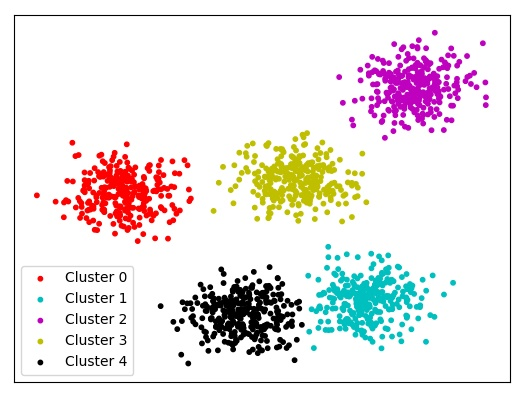
\includegraphics[width=1\linewidth]{cluster_result_graph.png}
	\end{center}
	\caption{聚类效果可视化}
	\label{word_vec:example}
\end{figure}

聚类的过程一般为以下步骤: \cite{DBLP:journals/csur/JainMF99,DBLP:journals/pami/JainDM00}
\begin{enumerate}
	\item 数据预处理: 文本处理中为词向量化和降维
	\item 特征值的选取:选出最能表示样本的特征,减少非特征值对样本的影响
	\item 特征值的过滤:去除样本中非特征值,保留特征值,并把筛选后的结果重新生产标准化数据。
	\item 进行聚类(或分组):根据样本的特征,选取合适的距离函数,也可创造新的距离函数,来衡量样本间的近似度,本项目中选取欧式距离作为距离函数。根据样本间的距离来进行分组
	\item 聚类质量评估:本项目使用轮廓系数评估、Calinski-Harabasz分数和相关性测试评估。
\end{enumerate}

本项目使用的聚类算法为Kmeans算法和GSDMM算法

\subsection{使用的技术工具与技术方法}

表\ref{main_tools}为本项目在聚类时主要使用的工具

\begin{table}[h!]
  \begin{center}
    \renewcommand\arraystretch{2}
    \begin{tabular}{|r|l|}
      \hline
      \textbf{类型} & \textbf{版本} \\
			\hline
			操作系统 & Ubuntu14.04.1 x86\_64 GNU/Linux  \\
			\hline
			编程语言 & Python 2.7.6 \\
			\hline
			虚拟环境管理器 & Pipenv version 2018.11.26 \\
			\hline
			\multirow{4}*{主要使用的python库} & jieba-0.39\\
			\cline{2-2}
			~ & sklearn-0.20.3 \\
			\cline{2-2}
			~ & numpy-1.16.2 \\
			\cline{2-2}
			~ & gensim-3.7.1 \\
			\hline
    \end{tabular}
    \caption{工具版本集合}
    \label{main_tools}
  \end{center}
\end{table} 

\subsection{Kmeans算法}

"Kmeans"一词最早是由Hugo Steinhaus在1957年提出,首次由James MacQueen于1967年使用\cite{macqueen1967},但是真正的标准算法,最早由Stuart Lloyd于1957年提出。在那时,Kmeans被用于脉冲编码调制技术,直到1982年才在贝尔实验室外发表\cite{Lloyd1056489}。在1965年,e.w.Forgy发表了本质上相同的方法,这就是为什么有时它被称为Lloyd-Forgy算法。

K-means方法是一种典型的空间聚类算法,它是一种无监督学习的方法。通常,无监督学习的输入数据是没有经过标注的。Kmeans方法通过研究样本在空间中的分布,以样本间的距离为标准,来把样本划分到若干个子集中,使得相同子集的样本间距离(interval)较小,不同子集的样本间的距离较大。通常由以下几种距离计算方式:欧氏距离、曼哈顿距离、切比雪夫距离和闵可夫斯基距离等。最常用的就是欧式距离(公式\ref{euclidean_distance}):

\begin{equation}
	\label{euclidean_distance}
	d\left( i, j \right) = \sqrt{\left[ \left( x_{i1} - x_{j1} \right)^2 + \left( x_{i2} - x_{j2} \right)^2 + \cdots + \left( x_{in} - x_{jn} \right)^2 \right]}
\end{equation}

Kmeans的流程如下:
\begin{enumerate}
	\item 首先给定预期类簇的数量K,即我们希望通过聚类获得K个类簇(组)
	\item 在样本集合中随机选取K个样本,作为每个类的中心,又称为质点,每个质点代表一个簇的的均值或者中心。
	\item\label{assign} 对于剩下的样本,计算每个样本与所有质点的距离,把每个样本分配到离它最近的质点所属簇的集合内。
	\item 经过步骤\ref{assign},每个簇都汇聚了一批样本。此时重新计算每个簇中所有样本的平均值形成的新质点。
	\item\label{should_end_kmeans} 如果新质点与老质点的距离小于一个预设的阈值(表明新质点的位置变化不大,该簇已趋于稳定收敛了),那么该类簇训练结束,算法终止。
	\item 若新老质点距离变化过大,则重复迭代\ref{assign}$\sim$\ref{should_end_kmeans}步,直到质点收敛,或者迭代次数达到预设的最大值为止。收敛函数为$E=\sum_{i=1}^{k} \sum_{p\in C_i} \left| p - m_i \right|^2$。$E$为所有样本的平方差之和,$p$为样本的空间向量,$m_i$为类$C_i$的平均值。
\end{enumerate}

遵循收敛函数的限制,迭代后簇将逐渐趋于紧凑,独立。

如流程图\ref{kmeans_process}所示:
\begin{figure}[H]
	\begin{center}
		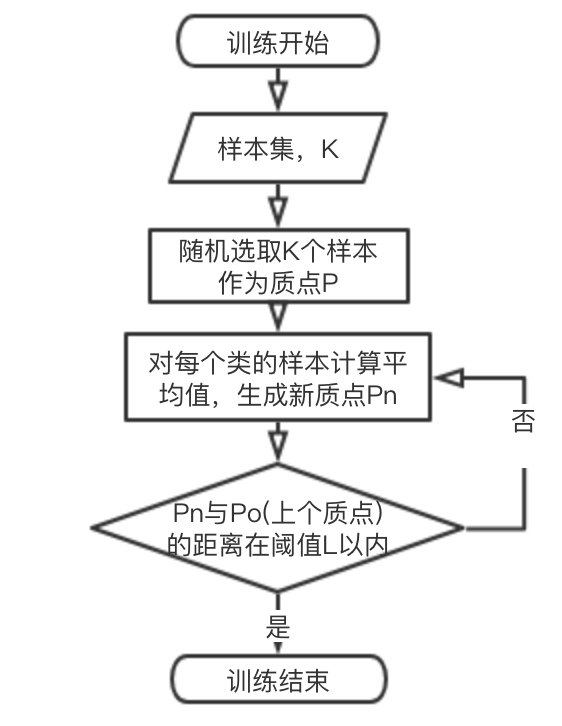
\includegraphics[width=.4\linewidth]{Kmeans_process.png}
	\end{center}
	\caption{kmeans聚类算法流程图}
	\label{kmeans_process}
\end{figure}


\subsection{GSDMM算法}
随着微博、Twitter和Facebook等社交媒体的普及,短文本聚类已经成为一项越来越重要的任务。由于短文本构建的词向量稀疏的特性,对短文本的聚类成为了一个很有挑战性的问题。面对这种情况,Jianhua Yin, Jianyong Wang于2014年发表了GSDMM(Gibbs Sampling for Dirichlet Multinomial Mixture 基于吉普斯采样的狄利克雷多项式混合算法)\cite{Yin:2014}。该算法基于狄利克雷多项式混合模型,提出了一种折叠吉布斯抽样(Gibbs Sampling)算法,这是因为对DMM模型的后验期望进行计算非常困难,所以J.Y和J.W采用了吉布斯抽样的方法。GSDMM能够自动推断数目,无需预设K值,还能在聚类结果的完全性和均匀性之间取得良好的平衡,并且收敛速度快。GSDMM还能处理短文本的稀疏性和高维性问题,并能获得每个聚类的代表词。

根据J.Y和J.W的广泛的实验研究表明\cite{Yin:2014},与其他三种聚类模型(Kmeans,Hac,DMAFP)相比,GSDMM的表现更佳,性能更好。它解决了短文本的稀疏和高维的问题,并且可以获得每个聚类的关键词。


\subsubsection{Movie Group Process}
J.Y和J.W假设,在一个电影讨论的课程上,教授计划将学生分成若干个小组。教授希望分组的结果是:每一组内的同学,与其组员所看过的相同的电影更多,以便他们有更多的共同话题。教授要求每个同学在几分钟之内写下他们所看过的电影,整理出一个列表。(列表不会太长,因为学生没有足够的时间写完所有的电影,他们更有可能写下他们最近看的电影或者他们非常喜欢的电影)现在,每个学生都能拿出一份电影清单了。教授需要想办法吧学生分成若干个小组,目标是同一组的学生的电影列表相似度更高,不同组之间学生的电影列表相似度最低。

现在把这个电影爱好分组问题与短文本聚类问题链接起来,输入是学生(文档),每个学生(文档)由电影的简短列表(单词)组成,目标是将学生(文档)分成几组,以便同一组中的学生(文档)相似,不同组中的学生(文档)不同。我们将电影(单词)的数量定义为V。短文本的稀疏特征意味着它非常大(通常大于105),而每个短文本中的平均字数(L)很小(通常小于102)

需要注意的是,Kmeans和HAC在做文本聚类的时候,通常使用的是词向量模型VSM(Vector Space Model)来向量化词,每个文本都使用长度为V的向量来表示,向量的每个元素是相应的字的权重(如TF-IDF)。由于短文本的词向量稀疏的问题,文档中大部分词的TF都=1,这意味着TF在短文本中的应用是无效的。经过每个间断的文档只有少量的单词,但它呈现的是一个大小约为V(通常大于105)的向量。这种词向量的表示通常会导致高时间复杂度和高空间复杂度。

继续电影讨论课程的问题,教授最终决定这样安排,他申请了一个足够大的教室,然后把学生们随机分配到K张桌子上,并让学生们重新选择一个桌子,她希望学生们选新桌子的时候遵循一下两条准则:

\begin{enumerate}
	\item 选择一个拥有更多学生的桌子
	\item 选择一个组员的电影清单与自己相似桌子
\end{enumerate}

随着学生们陆续重选好桌子,一些桌子的人数会越来越多,而一些桌子会逐渐没人乃至消失,我们的期望是最总只有一部分的桌子还有学生,并且这些桌子的组员有共同的电影爱好,换而言之,教授可以通过这种方法把学生分成几个组。

J.Y和J.W 将上述过程称为Movie Group Process(MGP)。我们可以看出,上述两个准则与聚类的两个目标有关:完整性和同质性\cite{DBLP:conf/emnlp/RosenbergH07}

GSDMM的详细证明和质量评估可以参考J.Y和J.W的\textbf{A Dirichlet Multinomial Mixture Model-based Approach forShort Text Clustering}\cite{Yin:2014}中的2.3章和2.4章

\subsection{本项目中的实际运用}

